\subsection{Cryptographic Primitives}

This section overviews the cryptosystems used by secure architectures. We are
interested in cryptographic primitives that guarantee privacy, integrity, and
freshness, and we treat these primitives as black boxes, focusing on their use
in larger systems. \cite{katz2014crypto} covers the mathematics behind
cryptography, while \cite{ferguson2011crypto} covers the topic of building
systems out of cryptographic primitives.

A message whose \textit{privacy} is protected can be transmitted over an
insecure medium without an adversary being able to obtain the information in
the message. When \textit{integrity} protection is used, the receiver is
guaranteed to either obtain a message that was transmitted by the sender, or to
notice that an attacker tampered with the message's content.

When multiple messages get transmitted over an untrusted medium, a
\textit{freshness} guarantee assures the receiver that she will obtain the
latest message coming from the sender, or will notice an attack. A freshness
guarantee is stronger than the equivalent integrity guarantee, because the
latter does not protect against \textit{replay attacks} where the attacker
replaces a newer message with an older message coming from the same sender.

These concepts might be better illustrated by the following example. Suppose
Alice is a wealthy investor who wishes to either \textbf{buy} or \textbf{sell}
an item every day. Alice cannot trade directly, and must relay her orders to
her broker, Bob, over a network connection owned by Eve.

A communication system with privacy guarantees would prevent Eve from
distinguishing between a \textbf{buy} and a \textbf{sell} order, as illustrated
in Figure~\ref{fig:privacy_attack}. Without privacy, Eve would know Alice's
order before it is is placed by Bob, so Eve would presumably gain a financial
advantage at Alice's expense.

\begin{figure}[hbt]
  \centering
  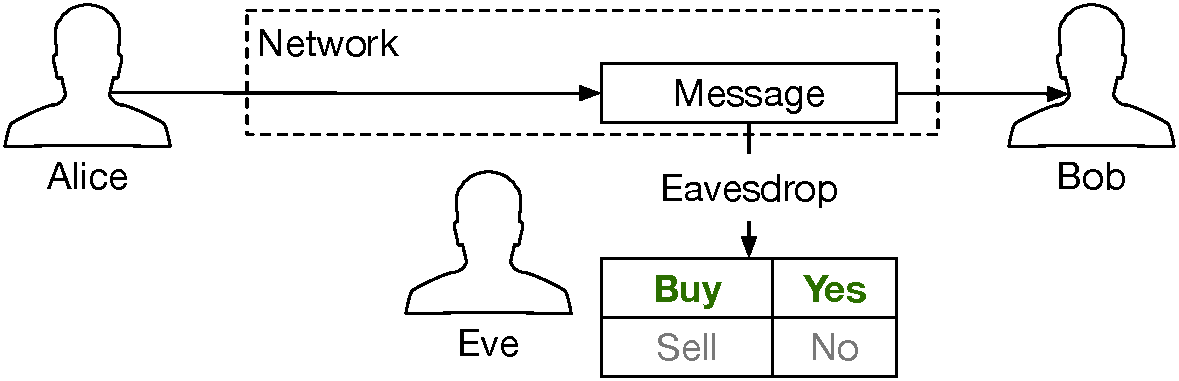
\includegraphics[width=85mm]{figures/privacy_attack.pdf}
  \caption{
    In a privacy attack, Eve sees the message sent by Alice to Bob and can
    understand the information inside it. In this case, Eve can tell that the
    message is a \textbf{buy} order, and not a \textbf{sell} order.
  }
  \label{fig:privacy_attack}
\end{figure}

A system with integrity guarantees would prevent Eve from replacing Alice's
message with a false order, as shown in Figure~\ref{fig:integrity_attack}. In
this example, without integrity guarantees, Eve could replace Alice's message
with a \textbf{sell-everything} order, and buy Alice's assets at a very low
price.

\begin{figure}[hbt]
  \centering
  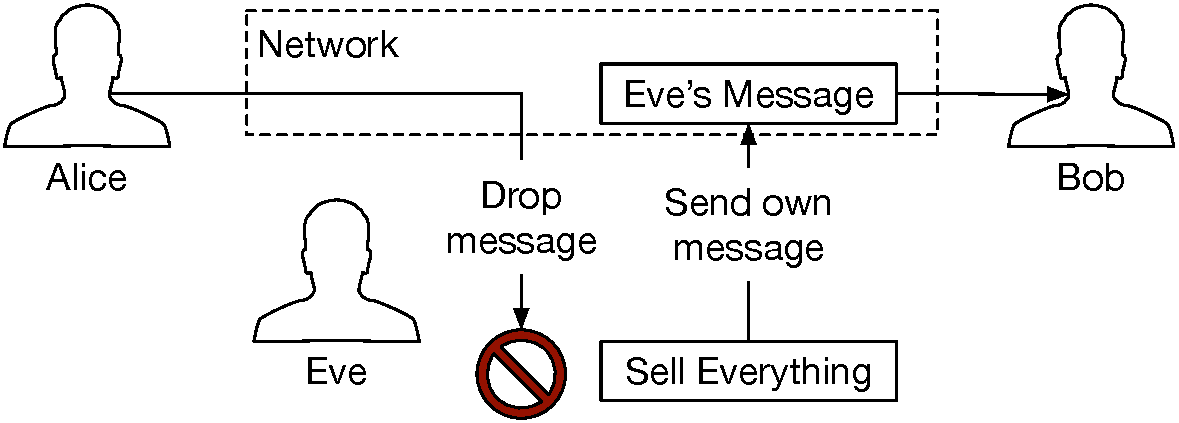
\includegraphics[width=85mm]{figures/integrity_attack.pdf}
  \caption{
    In an integrity attack, Eve replaces Alice's message with her own. In this
    case, Eve sends Bob a \textbf{sell-everything} order.
    understand the information inside it. In this case, Eve can tell that the
    message is a \textbf{buy} order, and not a \textbf{sell} order.
  }
  \label{fig:integrity_attack}
\end{figure}

Last, a communication system that guarantees freshness would ensure that Eve
cannot perform the replay attack pictured in Figure~\ref{fig:freshness_attack},
where she would replace Alice's message with an older message. Without
freshness guarantees, Eve could mount the following attack, which bypasses
both privacy and integrity guarantees. Over a few days, Eve would copy and
store Alice's messages from the network. As each order would reaches Bob, Eve
would observe the market and determine if the order was \textsc{buy} or
\textsc{sell}. After building up a database of messages labeled \textsc{buy} or
\textsc{sell}, Eve would replace Alice's message with an old message of her
choice.

\begin{figure}[hbt]
  \centering
  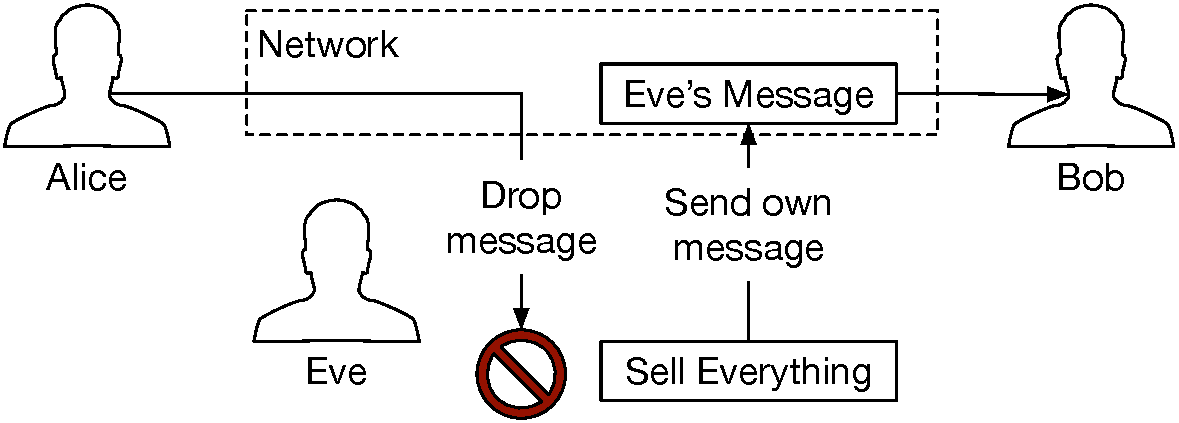
\includegraphics[width=85mm]{figures/integrity_attack.pdf}
  \caption{
    In a freshness attack, Eve replaces Alice's message with a message that she
    sent at an earlier time. In this example, Eve builds a database of labeled
    messages over time, and is able to send Bob her choice of a \textsc{buy} or
    a \textsc{sell} order.
  }
  \label{fig:freshness_attack}
\end{figure}


\subsubsection{Cryptographic Keys}

All cryptographic primitives that we describe here rely on \textit{keys}, which
are small pieces of information that must only be disclosed according to
specific rules. A large part of a system's security analysis focuses on
ensuring that the keys used by the underlying cryptographic primitives are
produced and handled according to the primitives' assumptions.

Each cryptographic primitive has an associated \textit{key generation
algorithm} that uses random data to produce a unique key. The random data is
produced by a \textit{cryptographically strong pseudo-random number generator}
(CSPRNG) that expands a small amount of \textit{random seed} data into a much
larger amount of data, which is computationally indistinguishable from true
random data. The random seed must be obtained from a true source of randomness
whose output cannot be predicted by an adversary, such as the least-significant
bits of the readings coming from a hardware temperature sensor.

\textit{Symmetric key} cryptography requires that all the parties in the system
establish a shared \textit{secret key}, which is usually referred to as ``the
key''. Typically, one party executes the key generation algorithm and securely
transmits the resulting key to the other parties, as illustrated in
Figure~\ref{fig:symmetric_key_generation}. The channel used to
distribute the key must provide privacy and integrity guarantees, which is a
non-trivial logistical burden. The symmetric key primitives mentioned here do
not make any assumption about the key, so the key generation algorithm simply
grabs a fixed number of bits from the CSPRNG.

\begin{figure}[hbt]
  \centering
  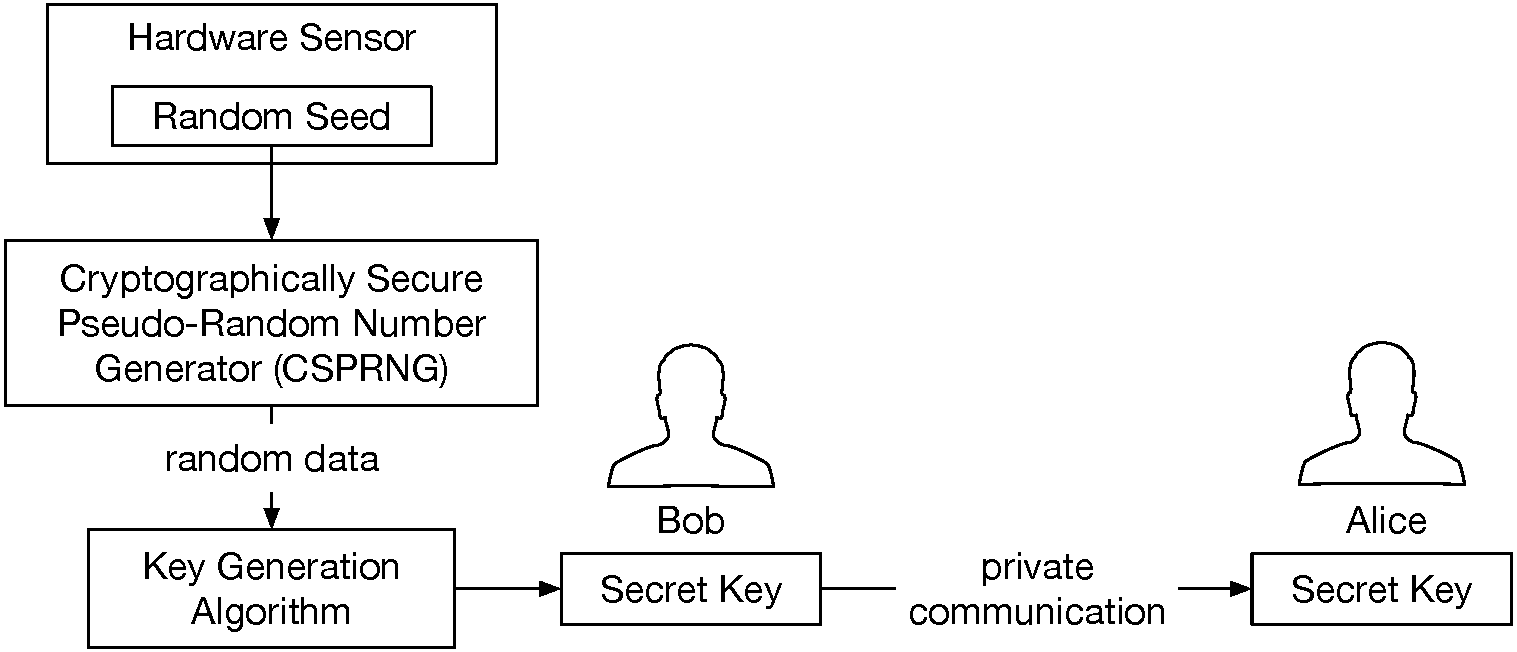
\includegraphics[width=87mm]{figures/symmetric_key_generation.pdf}
  \caption{
    In symmetric key cryptography, a secret key is shared by the parties that
    wish to communicate securely.
  }
  \label{fig:symmetric_key_generation}
\end{figure}

The salient feature of \textit{asymmetric key} cryptography is that it does not
require a private channel for key distribution. Each party executes the key
generation algorithm, which produces a \textit{private key} and a
\textit{public key} that are mathematically related. Each party's public key
is distributed to the other parties over a channel with integrity guarantees,
as shown in Figure~\ref{fig:asymmetric_key_generation}.
Asymmetric key primitives are more flexible than their symmetric key
counterparts, but are more complicated and consume more computational
resources.

\begin{figure}[hbt]
  \centering
  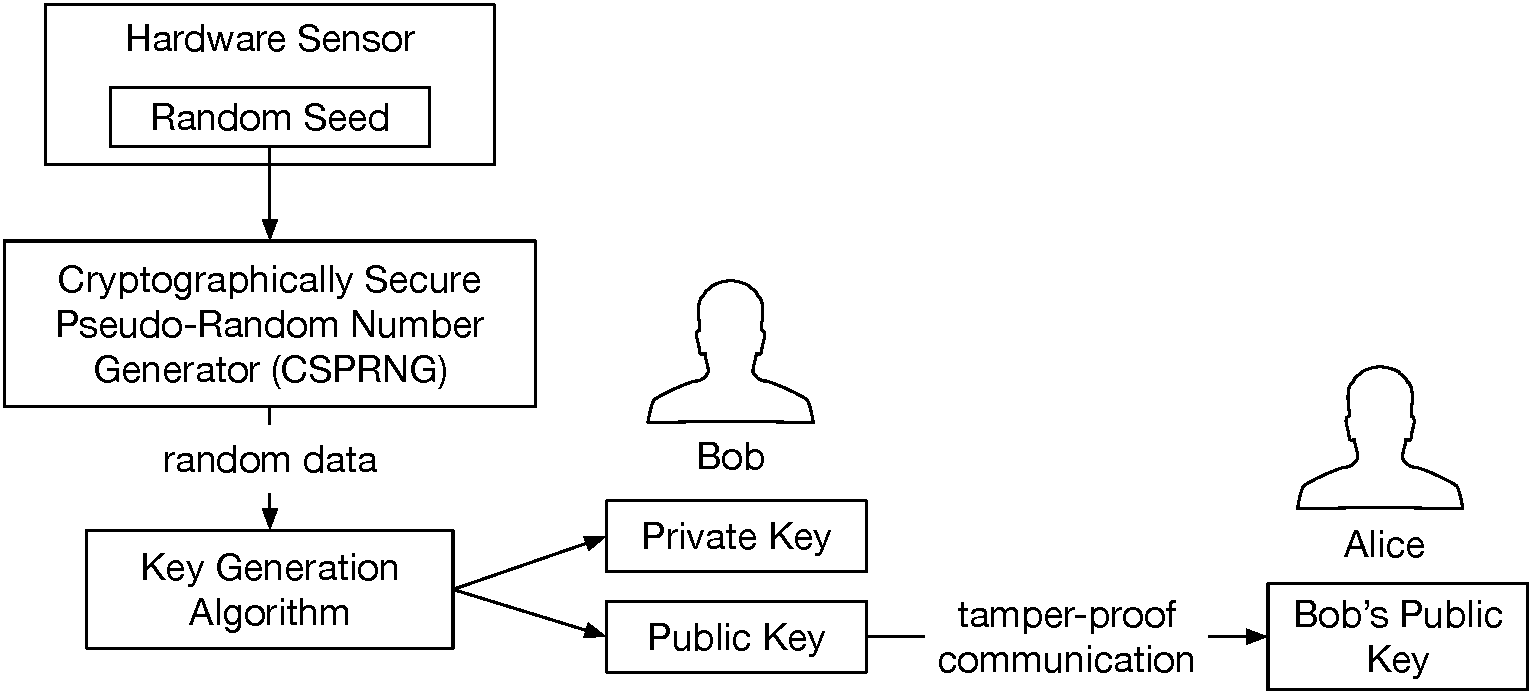
\includegraphics[width=87mm]{figures/asymmetric_key_generation.pdf}
  \caption{
    An asymmetric key generation algorithm produces a private key and an
    associated public key. The private key is held confidential, while the
    public key is given to any party who wishes to securely communicate with
    the private key's holder.
  }
  \label{fig:asymmetric_key_generation}
\end{figure}


\subsubsection{Privacy}

Privacy guarantees are obtained by applying an \textit{encryption algorithm} to
the sensitive information, as shown in Figures~\ref{fig:symmetric_encryption}
and~\ref{fig:asymmetric_encryption}. The original information can be recovered
from the encrypted output by running a \textit{decryption algorithm} with the
proper key. The information is hidden in the encrypted output in such a way
that an adversary cannot obtain it without the decryption key. Symmetric key
encryption schemes use the same secret key for encryption and decryption, while
asymmetric key encryption schemes use the public key for encryption, and the
corresponding private key for decryption.

\begin{figure}[hbt]
  \centering
  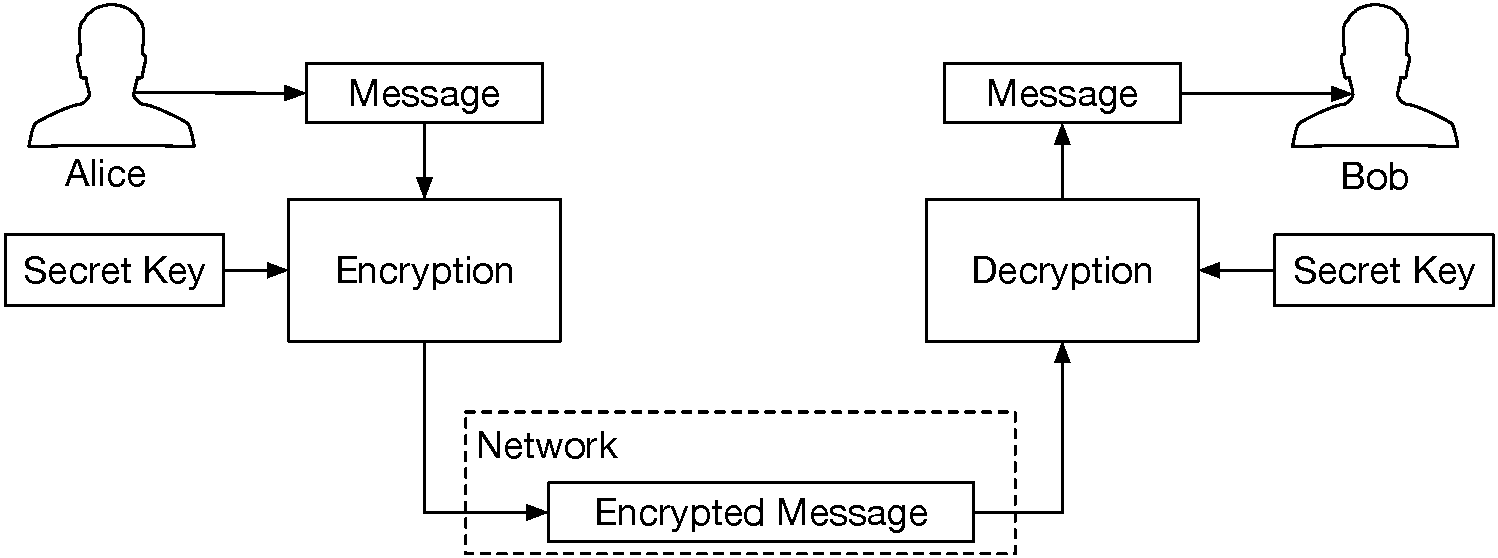
\includegraphics[width=87mm]{figures/symmetric_encryption.pdf}
  \caption{
    In a symmetric key encryption scheme, the same secret key must be provided
    to both the encryption and the decryption algorithm.
  }
  \label{fig:symmetric_encryption}
\end{figure}

\begin{figure}[hbt]
  \centering
  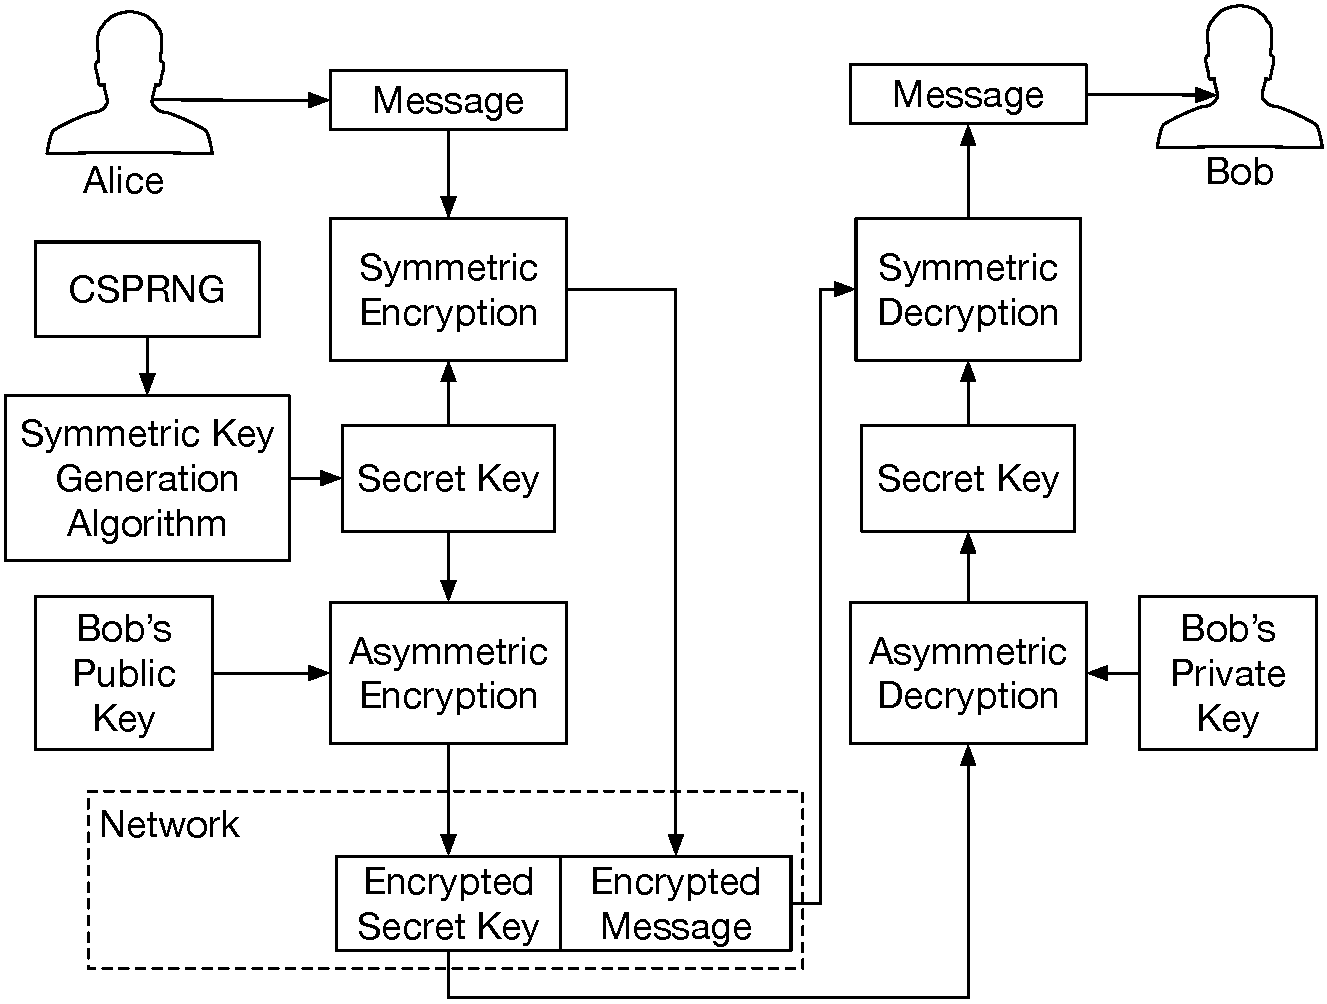
\includegraphics[width=87mm]{figures/asymmetric_encryption.pdf}
  \caption{
    In the asymmetric key setting, the encryption algorithm operates on a
    public key, and the decryption algorithm uses the corresponding private
    key.
  }
  \label{fig:asymmetric_encryption}
\end{figure}

At the time of this writing, the most popular choice of symmetric encryption
algorithm is the
\textit{American Encryption Standard}~(AES)~\cite{daemen1999aes}, which
operates on 128-bit keys. The most deployed asymmetric encryption system is
based on the \textit{Rivest-Shamir-Adelman}~(RSA)~\cite{rivest1978rsa}
algorithm. RSA has variable key sizes, and 2048-bit key pairs are considered to
provide the same security as 128-bit AES keys. Recently, elliptic curve
cryptography~\cite{koblitz1987ecc} has gained a surge in popularity, thanks to
its smaller key sizes. For example, a 256-bit ECC key is considered to have the
same security as a 2048-bit RSA key.


\subsubsection{Integrity}

Many cryptosystems that provide integrity guarantees are built upon
\textit{cryptographically strong hashing} functions. These hash functions
operate on an unbounded amount of input data and produce a small fixed-size
output. cryptographically strong hash functions have a few guarantees, such as
\textit{pre-image resistance}, which states that an adversary cannot produce
input data corresponding to a given hash output. The most popular cryptographic
hash function at the time of this writing is the
\textit{Secure Hashing Algorithm}~(SHA)~\cite{eastlake2001sha1}.

In the symmetric key setting, integrity guarantees are typically obtained using
an \textit{Hash Message Authentication Code}~(HMAC)~\cite{krawczyk1997hmac}
construction that combines a symmetric encryption algorithm, like AES, with a
cryptographically secure hash function, such as SHA. The message sender runs
the HMAC algorithm and sends the output HMAC value along with the original
message, as shown in Figure~\ref{fig:symmetric_hmac}. The message receiver
verifies that the received HMAC value is the same as the output of running the
HMAC algorithm on the message. HMAC algorithms inherit the pre-image resistance
property from their underlying cryptographic hash functions, and have the
additional property that an adversary cannot produce the correct HMAC for a
message without the secret key.

\begin{figure}[hbt]
  \centering
  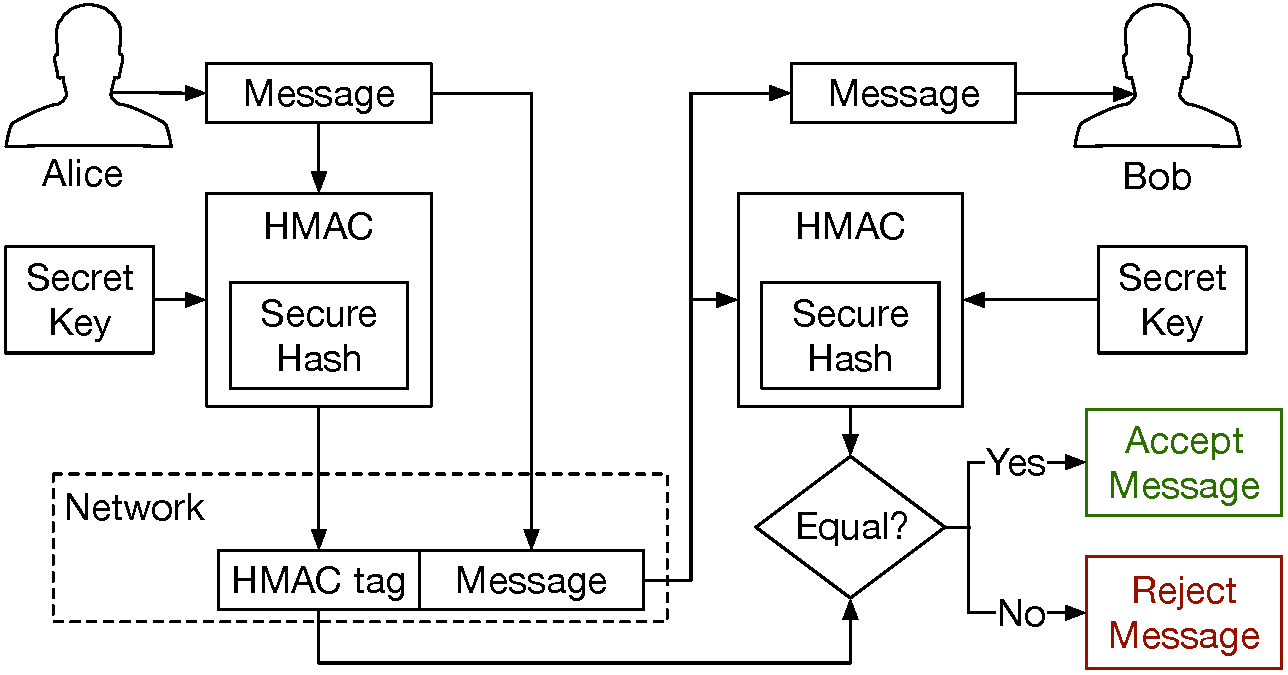
\includegraphics[width=87mm]{figures/symmetric_hmac.pdf}
  \caption{
    In the symmetric key setting, integrity is assured by computing a
    Hash-bassed Message Authentication Code (HMAC) and transmitting it over the
    network along the message. The receiver re-computes the HMAC and compares
    it against the version received from the network.
  }
  \label{fig:symmetric_hmac}
\end{figure}

Asymmetric key primitives that provide integrity guarantees are known as
\textit{signatures}. The message sender provides the private key to a
\textit{signing} algorithm, and transmits the output signature along with the
message, as shown in Figure~\ref{fig:asymmetric_signing}. The message receiver
feeds the public key and the signature to a \textit{signature verification}
algorithm, which returns \textsc{true} if the message matches the signature,
and \textsc{false} if the message has been tampered with.

\begin{figure}[hbt]
  \centering
  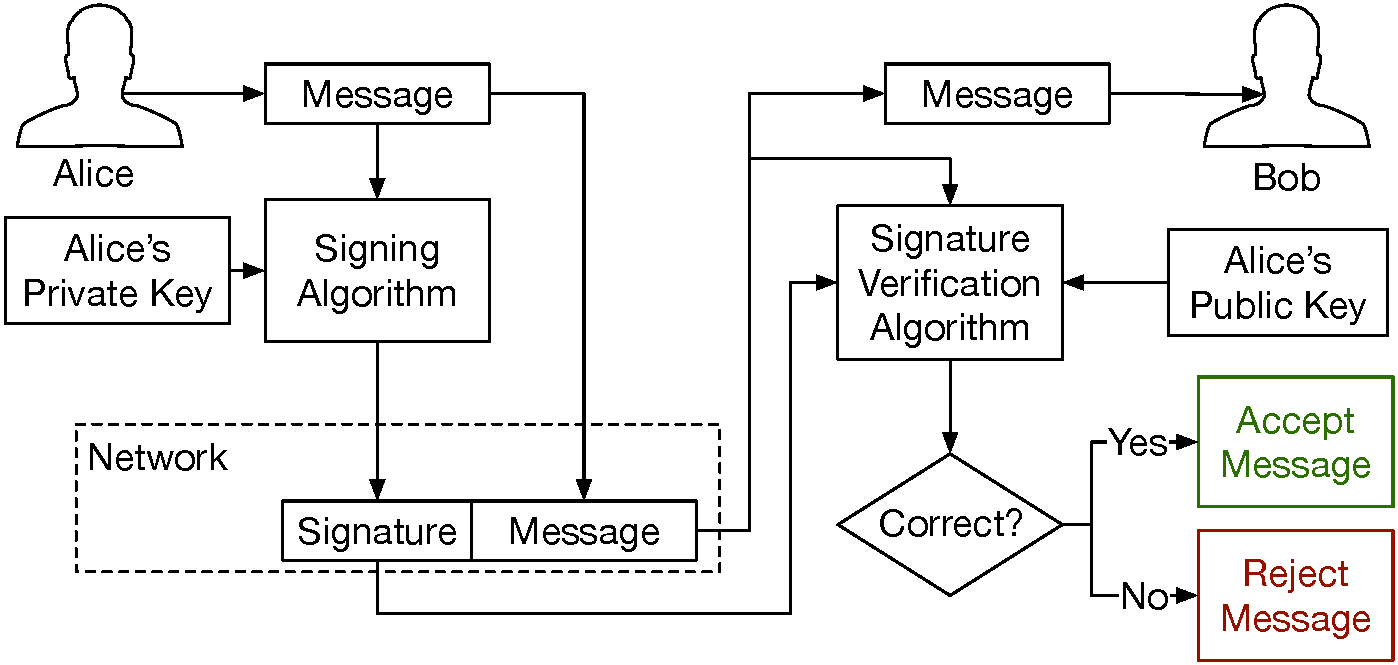
\includegraphics[width=87mm]{figures/asymmetric_signing.pdf}
  \caption{
    In the symmetric key setting, integrity is assured by computing a
    Hash-bassed Message Authentication Code (HMAC) and transmitting it over the
    network along the message. The receiver re-computes the HMAC and compares
    it against the version received from the network.
  }
  \label{fig:asymmetric_signing}
\end{figure}


Signing algorithms can only operate on small messages and are computationally
expensive. Therefore, in practice, the message to be transmitted is first ran
through a cryptographically strong hash function, and the hash is provided as
the input to the signing algorithm.

At the time of this writing, the most popular choice for providing encryption
in shared secret settings is a SHA-based HMAC function, and the most popular
signature algorithm is based on the RSA algorithm.


\subsubsection{Freshness}

In the network setting, freshness is ensured by adding unique pieces of
information to each message, which can be used by the receiver to detect replay
attacks. The unique information is either sequence numbers or \textit{nonces},
which are single-use random numbers.
